\newpage
\subsection*{ГЛ13 8}
\noindent
Докажем сперва вспомогательное утверждение\\
\begin{figure}[h]
	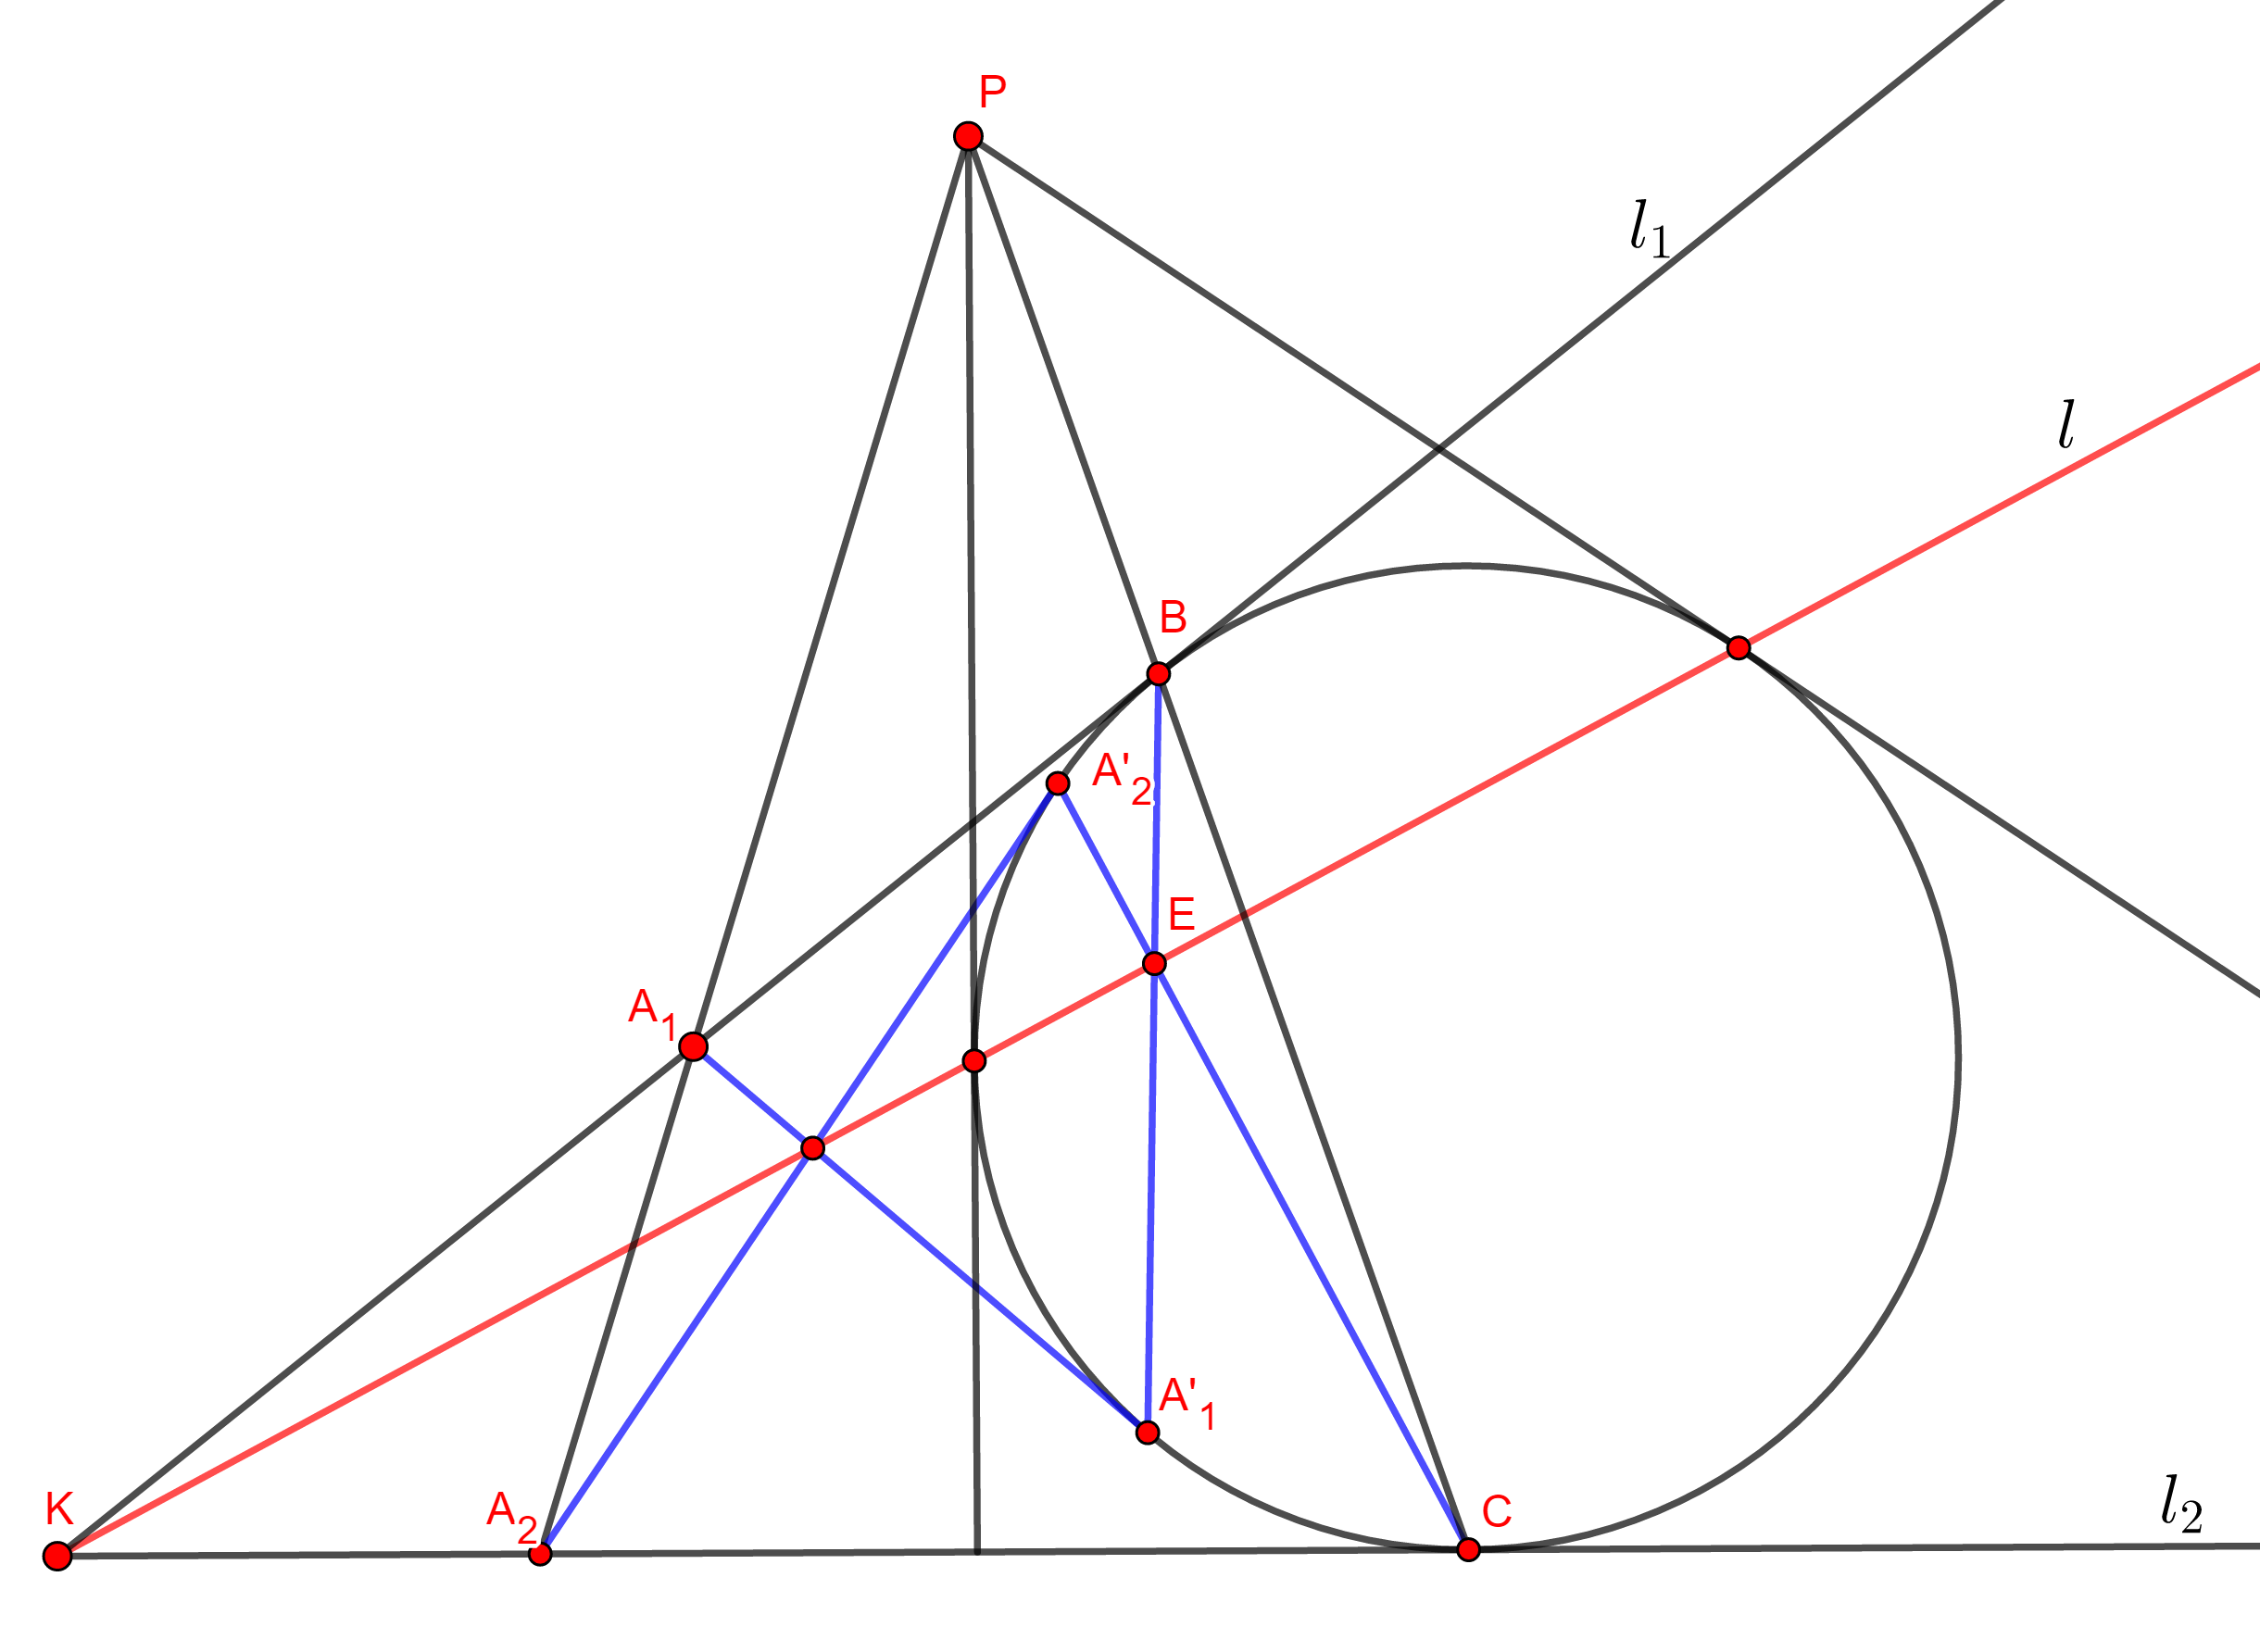
\includegraphics[width=0.5\linewidth]{pic24}
\end{figure}\\
$P$ -- полюс $l$, $B$ полюс $l_1$, $C$ полюс $l_2$, следовательно $P,B,C$ на одной прямой.\\
Рассмотрим гомографию $\varphi: l_1 \to l_2$.\\
$PA_1 \cap l_2 = A_2$, $A_1A_1'$ и $A_2A_2'$ -- касательные, $A_2'C$ поляра $A_2$, $A_1'B$ поляра $A_1$.\\
Следовательно $A_1'B \cap A_2'C \in l$, откуда $P \in A_1'A_2'$, $A_1A_1' \cap A_2A_2' = E$. Тогда поляра $E$ это $A_1'A_2'$ и $E \in l$. И $\varphi(A) = B$ гомография.\\
Также заметим что для всех коник, касающихся $l_1, l_2$ в $B,C$, точка $P$ будет совпадать, а следовательно все такие коники задают одну и ту же гомографию.

\vskip 0.2in
\noindent
Перейдем к задаче
\begin{figure}[h!]
	\begin{minipage}[h]{0.5\linewidth}
		Пусть $C_1$ -- большая коника, а $C_2$ -- меньшая.\\
		$PC \cap l_{\infty} = D$ и $CA,BA$ -- касательные к меньшей конике, $AC \cap l_{\infty} = A_0,\ CB \cap l_{\infty} = B_0$.\\
		Заметим что обе коники задают одну и ту же гомографию $\varphi: l_1 \to l_2$, а также $\varphi(I_1) = I_2,\ \varphi(I'_1) = I'_2$. $\varphi(P) = P$, $\varphi(A) = B$.\\
		Распишем равенства двойных отношений
		$[I'_1, I_1, D, A_0] = [I_3, I_2, P, B] = [I_2, I_3, B, P] = [I'_1, I_1, B_0, D]$, откуда следует равенство углов.
	\end{minipage}
	\hfill
	\begin{minipage}[h]{0.5\linewidth}
		\center{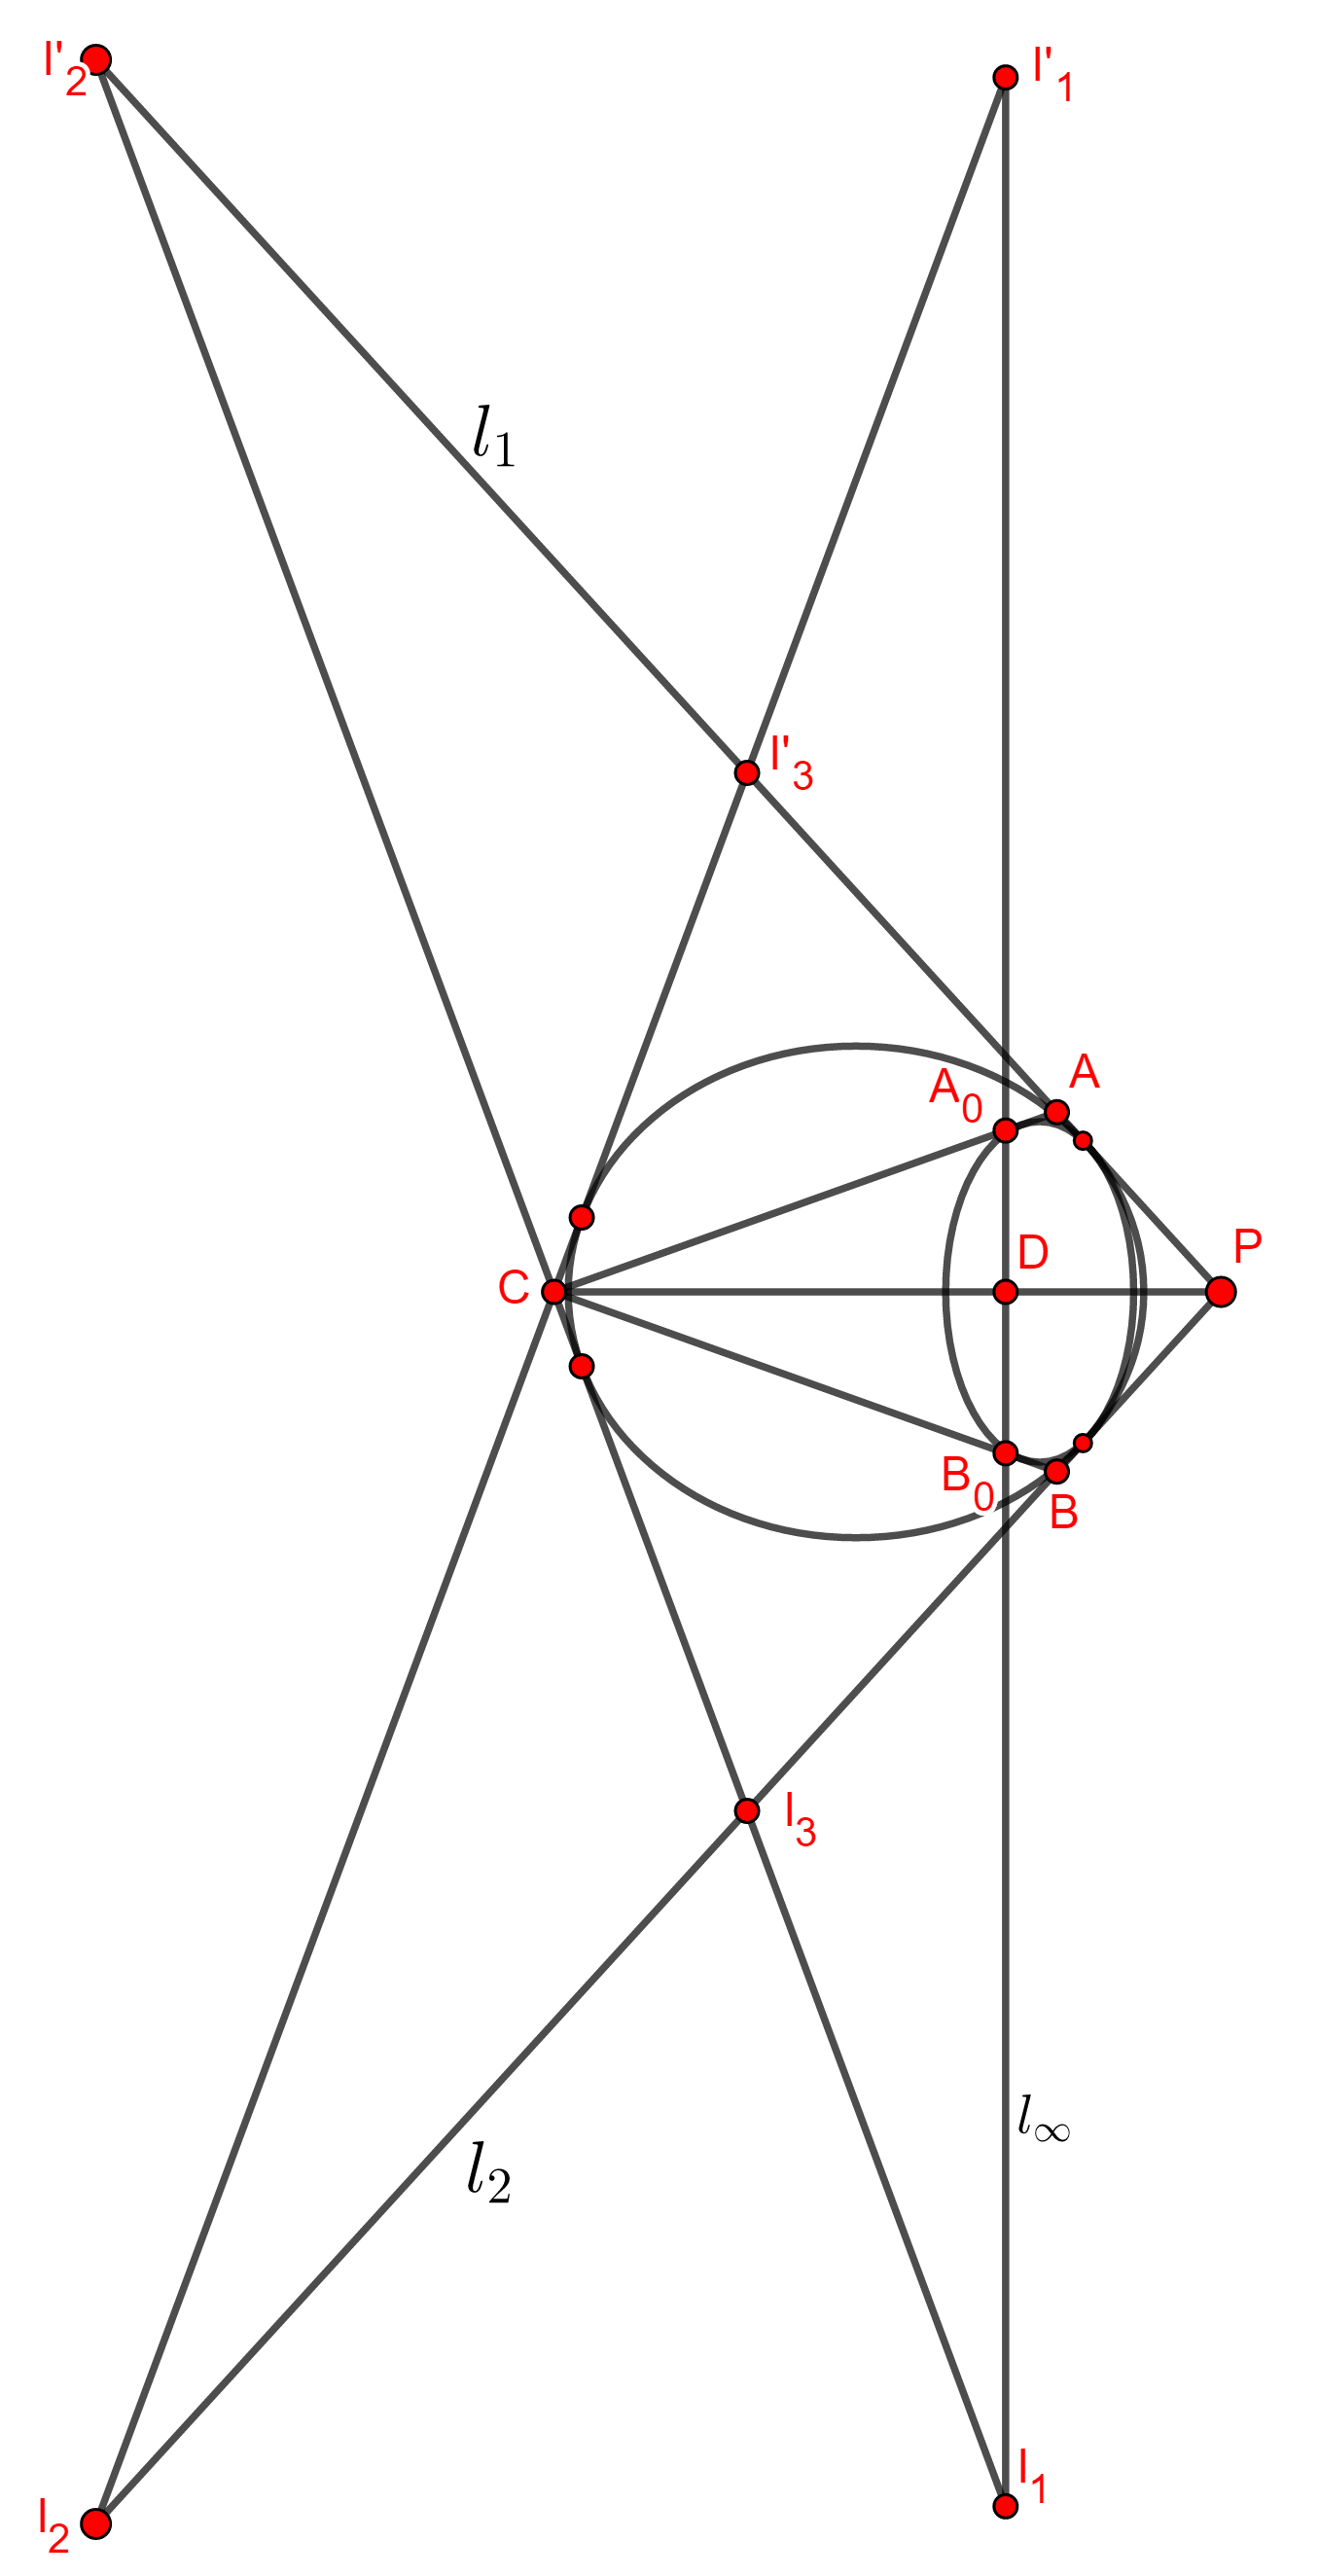
\includegraphics[width=0.78\linewidth]{pic25}}
	\end{minipage}
\end{figure}